% Created 2022-11-25 Fri 09:46
\documentclass[9pt, b5paper]{article}
\usepackage{xeCJK}
\usepackage{minted}
\usepackage[T1]{fontenc}
\usepackage[scaled]{beraserif}
\usepackage[scaled]{berasans}
\usepackage[scaled]{beramono}
\usepackage{graphicx}
\usepackage{xcolor}
\usepackage{multirow}
\usepackage{multicol}
\usepackage{float}
\usepackage{textcomp}
\usepackage{algorithm}
\usepackage{algorithmic}
\usepackage{latexsym}
\usepackage{natbib}
\usepackage{geometry}
\geometry{left=1.2cm,right=1.2cm,top=1.5cm,bottom=1.2cm}
\newminted{common-lisp}{fontsize=\footnotesize} 
\usepackage[xetex,colorlinks=true,CJKbookmarks=true,linkcolor=blue,urlcolor=blue,menucolor=blue]{hyperref}
\author{deepwaterooo}
\date{\today}
\title{Unity Export 导出到Android Studio再打包大致过程原理}
\hypersetup{
  pdfkeywords={},
  pdfsubject={},
  pdfcreator={Emacs 27.2 (Org mode 8.2.7c)}}
\begin{document}

\maketitle
\tableofcontents


\section{Unity 编译 Android 的原理解析和 apk 打包分析}
\label{sec-1}
\begin{itemize}
\item 最近由于想在Scene的脚本组件中,调用Android的Activity的相关接口,就需要弄明白Scene和Activity的实际对应关系,并对Unity调用Android的部分原理进行了研究。
\item 本文主要探讨Scene和Activity之间的关系,以及Unity打包apk和Android studio打包apk的差别在什么地方?找到这种差别之后,可以怎么运用起来?
\item 本文需要用到的工具:
\begin{itemize}
\item Android反编译工具——apktool
\item Android studio自带的反编译功能
\end{itemize}
\end{itemize}
\subsection{一、将Unity的Scene编译成apk,apk的程序入口会是什么?}
\label{sec-1-1}
\begin{itemize}
\item 新建一个Unity项目,创建一个Scene,将Unity工程编译打包成apk。
\item 对编译出来的apk,利用apktool进行反编译:apktool d unityTest.apk
\item 得到的AndroidManifest文件如下:
\end{itemize}
\begin{minted}[fontsize=\scriptsize,linenos=false]{xml}
<?xml version="1.0" encoding="utf-8" standalone="no"?>
<manifest
    xmlns:android="http://schemas.android.com/apk/res/android"
    android:installLocation="preferExternal"
    package="com.xfiction.p1"
    platformBuildVersionCode="25"
    platformBuildVersionName="7.1.1">

  <supports-screens
      android:anyDensity="true"
      android:largeScreens="true"
      android:normalScreens="true"
      android:smallScreens="true"
      android:xlargeScreens="true"/>

  <application
      android:banner="@drawable/app_banner"
      android:debuggable="false"
      android:icon="@drawable/app_icon"
      android:isGame="true"
      android:label="@string/app_name"
      android:theme="@style/UnityThemeSelector">

    <activity android:name="com.unity3d.player.UnityPlayerActivity" 

        android:configChanges="locale|fontScale|keyboard|keyboardHidden|mcc|mnc|navigation|orientation|screenLayout|screenSize|smallestScreenSize|touchscreen|uiMode"
        android:label="@string/app_name"
        android:launchMode="singleTask"
        android:screenOrientation="fullSensor">
      <intent-filter>
        <action android:name="android.intent.action.MAIN"/>
        <category android:name="android.intent.category.LAUNCHER"/>
        <category android:name="android.intent.category.LEANBACK_LAUNCHER"/>
      </intent-filter>
      <meta-data android:name="unityplayer.UnityActivity" android:value="true"/>
    </activity>
  </application>
  <uses-feature android:glEsVersion="0x00020000"/>
  <uses-feature android:name="android.hardware.touchscreen" android:required="false"/>
  <uses-feature android:name="android.hardware.touchscreen.multitouch" android:required="false"/>
  <uses-feature android:name="android.hardware.touchscreen.multitouch.distinct" android:required="false"/>
</manifest>
\end{minted}
\begin{itemize}
\item 由该AndroidManifest文件可知,系统仍然存在主Activity,名字为com.unity3d.player.UnityPlayerActivity。
\item 言下之意,编译只包含Scene的Unity工程,打包成Android apk,会以com.unity3d.player.UnityPlayerActivity作为主程序入口,那么问题来了,Scene如何加载显示到这个UnityPlayerActivity呢?
\end{itemize}
\subsection{二、UnityPlayerActivity如何加载Unity中的Scene?}
\label{sec-1-2}
\subsubsection{UnityPlayerActivity}
\label{sec-1-2-1}
\begin{itemize}
\item 这个就要从UnityPlayerActivity源码入手了,Android工程中使用UnityPlayerActivity需要依赖到Unity的Android插件classes.jar(位于Unity安装目录,可以用everything软件查找查找得到),对其进行反编译得到UnityPlayerActivity的部分源码:
\end{itemize}
\begin{minted}[fontsize=\scriptsize,linenos=false]{java}
public class UnityPlayerActivity extends Activity {
    protected UnityPlayer mUnityPlayer;
    protected void onCreate(Bundle var1) {
        this.requestWindowFeature(1);
        super.onCreate(var1);
        this.getWindow().setFormat(2);
        this.mUnityPlayer = new UnityPlayer(this);

        this.setContentView(this.mUnityPlayer); // <<<<<<<<<<<<<<<<<<<< 最终的界面显示需要依赖到UnityPlayer的实例

        this.mUnityPlayer.requestFocus();
    }
}
\end{minted}
\begin{itemize}
\item 虽然经过混淆,看起来比较费劲,但从代码this.setContentView(this.mUnityPlayer)可以看出,最终的界面显示需要依赖到UnityPlayer的实例。另外由于Google也做了一套Unity VR的SDK,与UnityPlayerActivity相对应的类,就是GoogleUnityActivity,下面也对它进行分析。
\end{itemize}
\subsubsection{从GoogleUnityActivity.java再入手分析}
\label{sec-1-2-2}
\begin{itemize}
\item GoogleUnityActivity是google推出的VR SDK中,用于实现Unity Activity的类,通过google查询其源码发现:1. GoogleUnityActivity.java实际上的布局文件activity\_main.xml
\end{itemize}
\begin{minted}[fontsize=\scriptsize,linenos=false]{xml}
<?xml version="1.0" encoding="utf-8"?>
<FrameLayout xmlns:android="http://schemas.android.com/apk/res/android"
    android:layout_width="match_parent"
    android:layout_height="match_parent" >
    <FrameLayout
        android:id="@+id/android_view_container"
        android:layout_width="match_parent"
        android:layout_height="match_parent"
        android:background="@android:color/transparent" />
</FrameLayout>
\end{minted}
\begin{itemize}
\item 布局文件中没有具体的内容,只包含一个FrameLayout布局。
\end{itemize}
\subsubsection{重点看GoogleUnityActivity的onCreate函数:}
\label{sec-1-2-3}
\begin{minted}[fontsize=\scriptsize,linenos=false]{java}
public class GoogleUnityActivity   extends Activity
    implements ActivityCompat.OnRequestPermissionsResultCallback {
    protected void onCreate(Bundle savedInstanceState) {
        requestWindowFeature(Window.FEATURE_NO_TITLE);
        super.onCreate(savedInstanceState);

        setContentView(R.layout.activity_main); // <<<<<<<<<<<<<<<<<<<< 这里是说可能会有两三种不同的实现方式吗?
        setContentView(R.id.activity_main.xml)

        mUnityPlayer = new UnityPlayer(this);
        if (mUnityPlayer.getSettings().getBoolean("hide_status_bar", true)) {
            getWindow().setFlags(WindowManager.LayoutParams.FLAG_FULLSCREEN,
                    WindowManager.LayoutParams.FLAG_FULLSCREEN);
        }
        ((ViewGroup) findViewById(android.R.id.content)).addView(mUnityPlayer.getView(), 0);
        mUnityPlayer.requestFocus();
    }
}
\end{minted}
\begin{itemize}
\item mUnityPlayer作为FrameLayoutView加入到view集合中进行显示,注意这里查找的id是android.R.id.content。根据官方对这个id的解释:android.R.id.content gives you the root element of a view, without having to know its actual name/type/ID. Check out Get root view from current activity
\item 由此可见,GoogleUnityActivity的实现原理,是创建一个只包含FrameLayout的空的帧布局,随后通过addView将UnityPlayer中的View加载到GoogleUnityActivity中进行显示。
\item 看起来跟UnityPlayerActivity有异曲同工之妙,两者牵涉的类都是UnityPlayer。
\end{itemize}
\subsubsection{UnityPlayer究竟是一个什么类呢?}
\label{sec-1-2-4}
\begin{itemize}
\item 对classes.jar包进行反编译得到UnityPlayer的部分代码:
\end{itemize}
\begin{minted}[fontsize=\scriptsize,linenos=false]{java}
public class UnityPlayer extends FrameLayout implements com.unity3d.player.a.a {
    public static Activity currentActivity = null;
    public UnityPlayer(ContextWrapper var1) {
        super(var1);
        if(var1 instanceof Activity) {
            currentActivity = (Activity)var1;
        }
    }
    public View getView() {
           return this;
    }
    public static native void UnitySendMessage(String var0, String var1, String var2);
    private final native boolean nativeRender();
    public void onCameraFrame(final com.unity3d.player.a var1, final byte[] var2) {
        final int var3 = var1.a();
        final Size var4 = var1.b();
        this.a(new UnityPlayer.c((byte)0) {
            public final void a() {
            UnityPlayer.this.nativeVideoFrameCallback(var3, var2, var4.width, var4.height);
                var1.a(var2);
            }
        });
    }
}
\end{minted}
\begin{itemize}
\item 从代码中可以发现:
\item UnityPlayer实际上是继承于FrameLayout;
\item 并且自带一个currentActivity的成员变量,在构造函数中,直接传入Activity的相关参数;
\item 在getView函数中直接返回该FrameLayout;
\item GoogleUnityActivity通过UnityPlayer的构造函数,将其context传递给UnityPlayer,并赋值给其成员变量currentActivity。
\item 由于UnityPlayer类做了混淆,关于渲染的核心功能也封装在native代码中,关于Scene转换到到UnityPlayer作为FrameLayout,只能做一个简单的推测:通过调用Android的GL渲染引擎,在native层进行渲染,并同步到FrameLayout在UnityPlayerActivity上进行显示。
\end{itemize}
\subsection{三、 如何将Scene显示在自定义的Activity当中(这里最好能找个真正的例子参考一下)}
\label{sec-1-3}
\begin{itemize}
\item 从以上研究的内容可知,假如要从要实现将Scene显示在固定的Activity当中,则需要对Activity的oncreate部分的countview和unityplayer进行处理。最简单的方法是写一个直接继承于UnityPlayerActivity或GoogleUnityActivity的类,并在类中写所需要的Unity调用Android的方法。这样Scene就会加载在特定的Activity当中,Unity c\#通过获取currentActivity变量就可以获取到该Activity,并调用其中的函数。
\end{itemize}
\subsection{四、 Unity Android 插件需要注意的问题}
\label{sec-1-4}
\begin{itemize}
\item Android studio工程包含多个module的依赖,则需要将对应的module编译的插件一起拷贝Plugins/Android/lib目录当中。
\item 在第一步骤下,可以直接删除打包后的aar library目录,尤其里面假如带有unity的Android插件classesjar,否则会编译报错。
\item 多个module编译的时候,注意manifest lablel相关设置,另外就是build.gradle的minSDKVersion信息。否则会出现manifest merger失败的错误。
\item 关于Unity的Android Manifest文件合并:Unity编写一个Scene,Android studio写一个包含主Activity的aar包,放在Plugins/Android目录当中。用Unity编译apk出来之后,反编译他的AndroidManifest文件,两个主Activity,默认显示包含Scene的Activity。解决方法:Unity的Manifest文件合并,把一个manifest放到Plugins/Android目录下,就不会合并manifest了。
\end{itemize}
\subsection{五、Unity打包Android apk的结构探究}
\label{sec-1-5}
\begin{itemize}
\item 由于Unity开发Android时,常常设计到Unity + Visual和Android studio的环境切换,Unity的开发往往会更快一些,更多的是Android java侧的代码编写和调试。
\item 这种情况时,有没有一种方法,能够将Unity编译好的Unity Scene和c\#相关文件,放到Android studio中进行打包,从而实现直接在Android studio中进行调试?
\item 方法原理倒是很简单,通过对比Unity打包的apk,与普通的Android apk的文件差别,找出Unity文件存放的目录,随后对应存放到Android studio工程目录中,最后通过Android studio完成对Unity相关文件的打包。
\item 首先将apk添加zip的后缀,方便用beyond compare进行对比:
\item 发现只是多了assert/bin目录,在这个目录之下,可以看到unity相关dll库
\item 将该文件,拷贝到Android studio工程的src/main/assert目录之下;
\item 在Android studio调试时,可以将aar library工程设置为app工程,这样就可以编译apk运行到手机了。
\item 用Android studio对该工程进行编译,发现assert/bin目录成功被打包进去。
\item 直接apk install 运行,可以看到跟Unity编译打包的apk,是相同的效果。
\item 相反,假如Android工程调试好之后,则直接编译成app模式修改成library模式,进行build之后,就会生成aar库,此时将aar库拷贝到Plugins/Android/lib目录当中,注意要删除aar库中的assert/bin,因为这个目录是我们先前从Unity拷贝过去的,假如不删除,在unity里面会出现重复打包导致的文件冲突的情况。
\item 由于当将Unity打包之后的bin目录拷贝到Android studio工程之后,Android studio此时是一个library工程,需要转换为app工程。关于这其中涉及到的Android studio library和app的转换,通过设置build.gradle文件来实现:
\item app模式:apply plugin: 'com.android.application'
\item library模式:apply plugin:   'com.android.library'
\item 不过在设置这两种模式时,需要注意applicationId "com.example.yin.myapplication"的设置,假如是library模式,则需要直接注释掉。
\item 假如Android的java部分重新调试好之后,重新将app模式改成library模式,进行build,将生成的aar包,拷贝到Unity Android Plugin目录中,就可以直接在Unity看运行效果了。 \textbf{不过一定要记得删除Android studio打包的aar文件里面的assert/bin目录,以防止在Unity中重复打包。}
\end{itemize}
\subsection{四、结论:}
\label{sec-1-6}
\begin{itemize}
\item Unity中的Scene在Android中,其实对应于Activity的FrameLayout,每个Scene的运行都有其Activity环境,通过currentActivity变量可以获取得到。
\item 要实现自定义的Activity能够具备直接加载Scene的功能,则需要其继承于UnityPlayerActivity或者GoogleUnityActivity,再或者,直接自定义实现UnityActivity类。
\item 提升Unity+Android Plugin项目开发效率的方法:● 直接将Unity打包的apk中的assert/bin目录拷贝到Android studio工程的src/main/assert目录当中,并且将Android工程配置成app模式,就可以直接在Android studio上面,对整个Unity+android plugin的工程进行调试。● Android studio部分调试好之后,需要修改build.gradle文件,重新将app模式修改为library模式,编译出aar包文件,删除原来拷贝过来的unity部分,放入到unity的Plugins/Android/lib目录下进行使用即可。
\end{itemize}

\section{Unity构建安卓原理详解}
\label{sec-2}
\begin{itemize}
\item 构建系统
\item Unity 支持两个 Android 构建系统:\_\_Gradle\_\_ 和 Internal。
\item Android 构建过程所涉及的步骤如下:
\begin{itemize}
\item 准备和构建 Unity 资源。
\item 编译脚本。
\item 处理插件。
\item 将资源拆分为放入 APK 和 OBB 的各个部分(如果已选择 \_\_Split Application Binary\_\_)。
\item 使用 AAPT 实用程序构建 Android 资源(仅限内部构建)。
\item 生成 Android 清单。
\item 将库清单合并到 Android 清单中(仅限内部构建)。
\item 将 Java 代码编译为 Dalvik 可执行文件格式 (DEX)(仅限内部构建)。
\item 构建 IL2CPP 库(如果已选择 \_\_IL2CPP Scripting Backend\_\_)。
\item 构建并优化 APK 和 OBB 包。
\end{itemize}
\item Gradle 构建系统
\begin{itemize}
\item Gradle 构建系统使用 Gradle 来构建 APK 或以 Gradle 格式导出项目,然后可以将其导入 Android Studio。选择此构建系统时,Unity 将执行与 Internal 构建系统相同的步骤,但不包括使用 AAPT 进行资源编译、合并清单以及运行 DEX。然后,Unity 生成 build.gradle 文件(以及其他所需的配置文件),并调用 Gradle 可执行文件,在此过程中向其传递任务名称和工作目录。最后,由 Gradle 构建 APK。
\item 有关更多详细信息,请参阅 Gradle for Android。
\end{itemize}
\item Internal 构建系统
\begin{itemize}
\item Internal 构建系统使用 Android SDK 实用程序创建 APK,从而构建并优化 APK 和 OBB 包。
\end{itemize}
\end{itemize}

\section{Unity是怎么打包APK文件的}
\label{sec-3}
\begin{itemize}
\item 在Unity里面有几个特殊的文件夹是跟打包APK有关的。首先我们就来了解一下,这些文件夹里面的内容是经历了哪些操作才被放到APK里面的呢?
\item 在Unity的Assets目录下,Plugins/Android无疑是其中的重中之重,首先我们先来看一个常见的Plugins/Android目录是什么样子的。
\end{itemize}
\begin{minted}[fontsize=\scriptsize,linenos=false]{tex}
-Android
-- ApolloBase
-- ApolloPlugins
-- assets
-- libs
-- res
-- AndroidManifest.xml
\end{minted}
\begin{itemize}
\item 后面的四个是Android工程的文件。前面两个文件夹是我们引用的第三方库,他们也会被打包到APK中。我们这个时候如果点进去前两个文件夹,我们会发现他们的目录结构跟Android这个目录也很像,大概是一下这个样子的。
\end{itemize}
\begin{minted}[fontsize=\scriptsize,linenos=false]{tex}
-ApolloPlugins
-- libs
-- res
-- AndroidManifest.xml
-- project.properties
\end{minted}
\begin{itemize}
\item 比较上下两层的目录接口我们可以发现有很多相似的部分,如:libs、res、assets文件夹以及AndroidManifest.xml文件。这些其实都是一个标准的Android项目的所需要的文件。Unity自带的Android打包工具的作用就是把上述这几个文件夹里面的内容以固定的方式组织起来压缩到APK文件里面。
\end{itemize}
\subsection{Android打包工具都会做什么样的操作。}
\label{sec-3-1}
\begin{itemize}
\item ● \textbf{libs文件夹里面有很多.jar文件} ,以及被放在固定名字的文件夹里面的.so文件。*.jar文件是Java编译器把.java代码编译后的文件,Android在打包的时候会把项目里面的所有jar文件进行一次合并、压缩、重新编译变成classes.dex文件被放在APK根目录下。当应用被执行的时候Android系统内的Java虚拟机(Dalvik或者Art),会去解读classes.dex里面的字节码并且执行。把众多jar包编译成classes.dex文件是打包Android应用不可或缺的一步。
\begin{itemize}
\item 看到这里有人可能会想不对啊,这一步只将jar包打成dex文件,那之前的java文件生成jar文件难道不是在这一步做吗?没错,这里用的jar包一般是由其他Android的IDE生成完成后再拷贝过来的。本文后面的部分会涉及到怎么使用Android的IDE并且生成必要的文件。
\end{itemize}
\item ● \textbf{libs文件夹的}.so文件* 则是可以动态的被Android系统加载的库文件,一般是由C/C++撰写而成然后编译成的二进制文件。要注意的是,由于实际执行这些二进制库的CPU的架构不一样,所以同样的CC++代码一般会针对不同的CPU架构生成几分不同的文件。这就是为什么libs文件夹里面通常都有armeabi-v7a、armeabi、x86等几个固定的文件夹,而且里面的.so文件也都是有相同的命名方式。Java虚拟机在加载这些动态库的时候会根据当前CPU的架构来选择对应的so文件。有时候这些so文件是可以在不同的CPU架构上执行的,只是在不对应的架构上执行速度会慢一些,所以当追求速度的时候可以给针对每个架构输出对应的so文件,当追求包体大小的时候输出一个armeabi的so文件就可以了。
\item ● \textbf{assets文件夹} ,这个里面的东西最简单了,在打包APK的时候,这些文件里面的内容会被原封不动的被拷贝到APK根目录下的assets文件夹。这个文件夹有几个特性。
\begin{itemize}
\item √ 里面的文件基本不会被Android的打包工具修改,应用里面要用的时候可以读出来。
\item √ 打出包以后,这个文件夹是只读的,不能修改。
\item √ 读取这个文件夹里面的内容的时候要通过特定的Android API来读取,参考getAssets()。
\item √ 基于上述两点,在Unity中,要读取这部分内容要通过WWW来进行加载。
\item 除了Plugins/Android内的所有assets文件夹里面的文件会连同StreamingAssets目录下的文件一起被放到APK根目录下的assets文件夹。
\end{itemize}
\item ● \textbf{res文件夹} 里面一般放的是xml文件以及一些图片素材文件。xml文件一般来说有以下几种:
\begin{itemize}
\item √ 布局文件,被放在res中以layout开头的文件夹中,文件里描述的一般都是原生界面的布局信息。由于Unity游戏的显示是直接通过GL指令来完成的,所以我们一般不会涉及到这些文件。
\item √ 字符串定义文件,一般被放到values文件夹下,这个里面可以定义一些字符串在里面,方便程序做国际
\item 化还有本地化用。当然有时候被放到里面的还有其他xml会引用到的字符串,一般常见的是app的名称。
\item √ 动画文件,一般定义的是Android原生界面元素的动画,对于Unity游戏,我们一般也不会涉及他。
\item √ 图片资源,一般放在以drawable为开头的文件夹内。这些文件夹的后缀一般会根据手机的像素密度来来进行区分,这样我们可以往这些文件夹内放入对应像素密度的图片资源。
\item 例如后缀为ldpi的drawable文件夹里面的图片的尺寸一般来说会是整个系列里面最小的,因为这个文件夹的内容会被放到像素密度最低的那些手机上运行。而一般1080p或者2k甚至4k的手机在读取图片的时候会从后缀为xxxxhdpi的文件夹里面去读,这样才可以保证应用内的图像清晰。图片资源在打包过程中会被放到APK的res文件夹内的对应目录。
\item √ Android还有其他一些常见的xml文件,这里就不一一列举了。
\item res文件夹下的xml文件在被打包的时候会被转换成一种读取效率更高的一种特殊格式(也是二进制的格式),命名的时候还是以xml为结尾被放到APK包里面的res文件夹下,其目录结构会跟打包之前的目录结构相对应。
\item 除了转换xml之外,Android的打包工具还会把res文件夹下的资源文件跟代码静态引用到的资源文件的映射给建立起来,放到APK根目录的resources.arsc文件。这一步可以确保安卓应用启动的时候可以加载出正确的界面,是打包Android应用不可或缺的一步。
\end{itemize}
\item ● \textbf{AndroidManifest.xml} ,这份文件太重要了,这是一份给Android系统读取的指引,在Android系统安装、启动应用的时候,他会首先来读取这个文件的内容,分析出这个应用分别使用了那些基本的元素,以及应该从classes.dex文件内读取哪一段代码来使用又或者是应该往桌面上放哪个图标,这个应用能不能被拿来debug等等。在后面的部分会有详细解释。打包工具在处理Unity项目里面的AndroidManifest文件时会将所有AndroidManifest文件的内容合并到一起,也就是说主项目引用到的库项目里面如果也有AndroidManifest文件,都会被合并到一起。这样就不需要手动复制粘贴。需要说明的是,这份文件在打包Android程序的时候是必不可少的,但是在Unity打包的时候,他会先检查Plugins目录下有没有这份文件,如果没有就会用一个自带的AndroidManifest来代替。此外,Unity还会自动检查项目中AndroidManifest里面的某些信息是不是默认值,如果是的话,会拿Unity项目中的值来进行替换。例如,游戏的App名称以及图标等。
\item ● \textbf{project.properties} ,这份文件一般只有在库项目里面能看得到,里面的内容极少,就只有一句话android.library=true。但是少了这份文件Android的打包工具就不会认为这个文件夹里面是个Android的库项目,从而在打包的时候整个文件夹会被忽略。这有时候不会影响到打包的流程,打包过程中也不会报错,但是打出的APK包缺少资源或者代码,一跑就崩溃。关于这份文件,其实在Unity的官方文档上并没有详细的描述(因为他实际上是Android项目的基础知识),导致很多刚刚接触Unity-Android开发的开发者在这里栽坑。曾经有个很早就开始用Unity做Android游戏的老前辈告诉我要搞定Unity中的Android库依赖的做法是用Eclipse打开Plugins/Android文件夹,把里面的所有的项目依赖处理好就行了。殊不知这样将Unity项目跟Eclipse项目耦合在一起的做法是不太合理的,会造成Unity项目开启的时候缓慢。
\item ● \textbf{其他文件夹例如aidl以及jni} 在Unity生成APK这一步一般不会涉及到,这里不展开。
\item 看到了上述介绍的Unity打包APK的基础知识我们知道了往Plugins/Android目录下放什么样的文件会对APK包产生什么样的影响。但是实际上上述的内容只是着重的讲了Unity是怎么打包APK,所以接下来会简述一下打包这个步骤到底是怎么完成的。
\item \textbf{Android提供了一个叫做aapt的工具,这个工具的全称是Android Asset Packaging Tool} ,这个工具完成了上述大部分的对资源文件处理的工作,而Unity则是通过对Android提供的工具链(Android Build Tools)的一系列调用从而完成打包APK的操作。这里感觉有点像我们写了个bat/bash脚本,这个脚本按照顺序调用Android提供的工具一样。在一些常见的Android IDE里面,这样的“bat/bash脚本”往往是一个完整的构建系统。最早的Android IDE是Eclipse,他的构建系统是Ant,是基于XML配置的构建系统。后来Android团队推出了Android专用的IDE——Android Studio(这个在文章后面会有详述),他的构建系统则是换成了gradle,从基于xml的配置一下子升级到了语言(DSL, Domain Specific Language)的层级,给使用Android Studio的人带来更多的弹性。
\item 写到这里我想很多人都清楚了要怎么把Android的SDK/插件放到Unity里面并且打包到Unity里面。这时候应该有人会说,光会放这些文件不够啊,我还需要知道自己怎么写Android的代码并且输出相应的SDK/插件给Unity使用啊。1
\end{itemize}

\section{unity3d 打包发布篇--MONO和IL2CPP原理}
\label{sec-4}
\begin{itemize}
\item 两种方式打包以后的项目目录结构
\end{itemize}

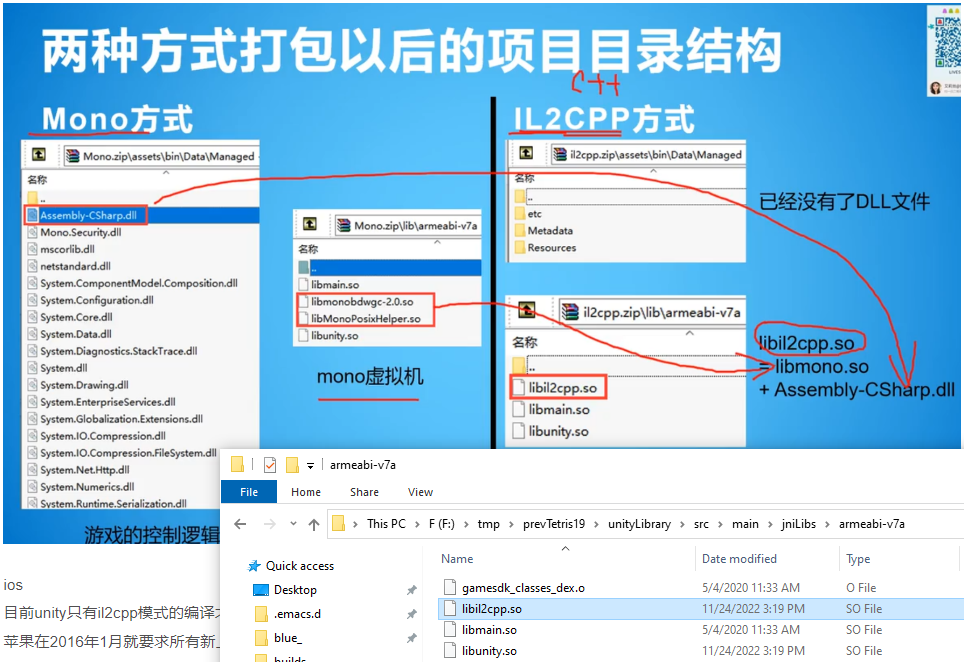
\includegraphics[width=.9\linewidth]{./pic/notes_20221125_094114.png}
\subsection{Mono方面}
\label{sec-4-1}

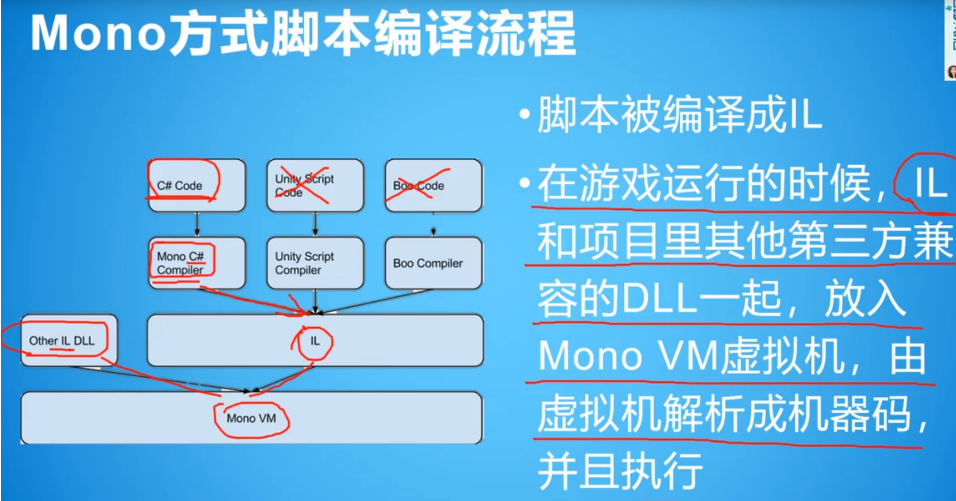
\includegraphics[width=.9\linewidth]{./pic/notes_20221125_094154.png}
\begin{itemize}
\item mono是一款开源、免费、可定制的跨平台.NET运行环境。由于.net只能在windows,mono相当于是一个.net CLR的跨平台变种,就是为了解决跨平台的移植问题。
\item 在运行IL方面上,热更也需要基于JIT,安卓支持即时编译JIT,虽然热更方便,但如果代码中有病毒木马,也一样编译。
\end{itemize}

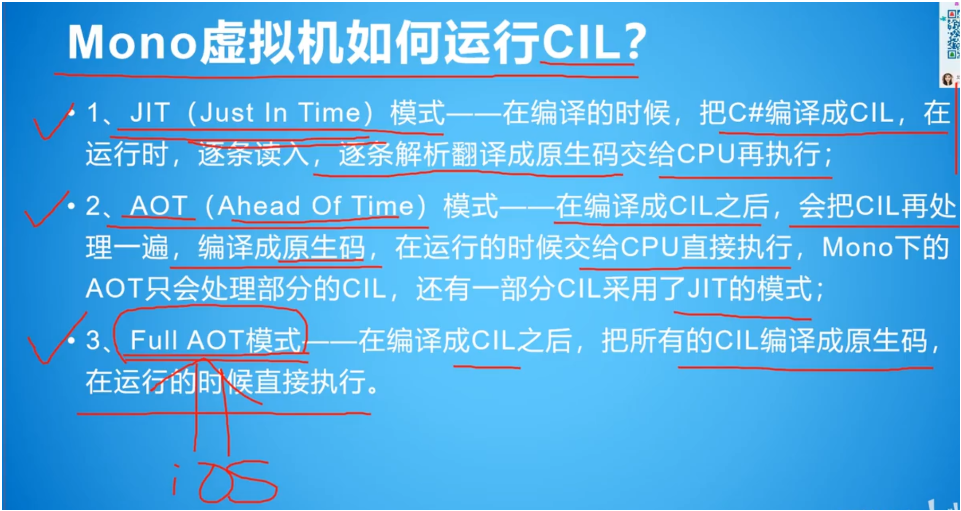
\includegraphics[width=.9\linewidth]{./pic/notes_20221125_094222.png}
\subsection{IL2CPP:}
\label{sec-4-2}

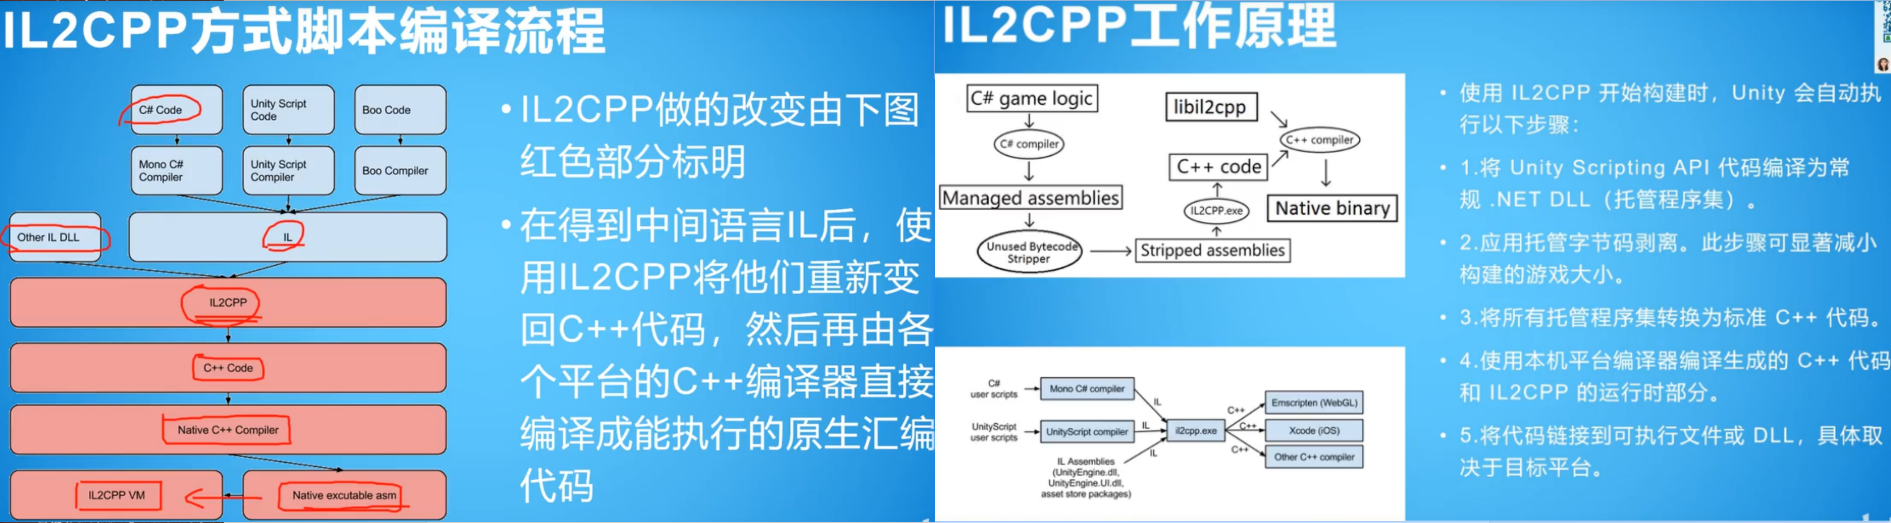
\includegraphics[width=.9\linewidth]{./pic/notes_20221125_094415.png}

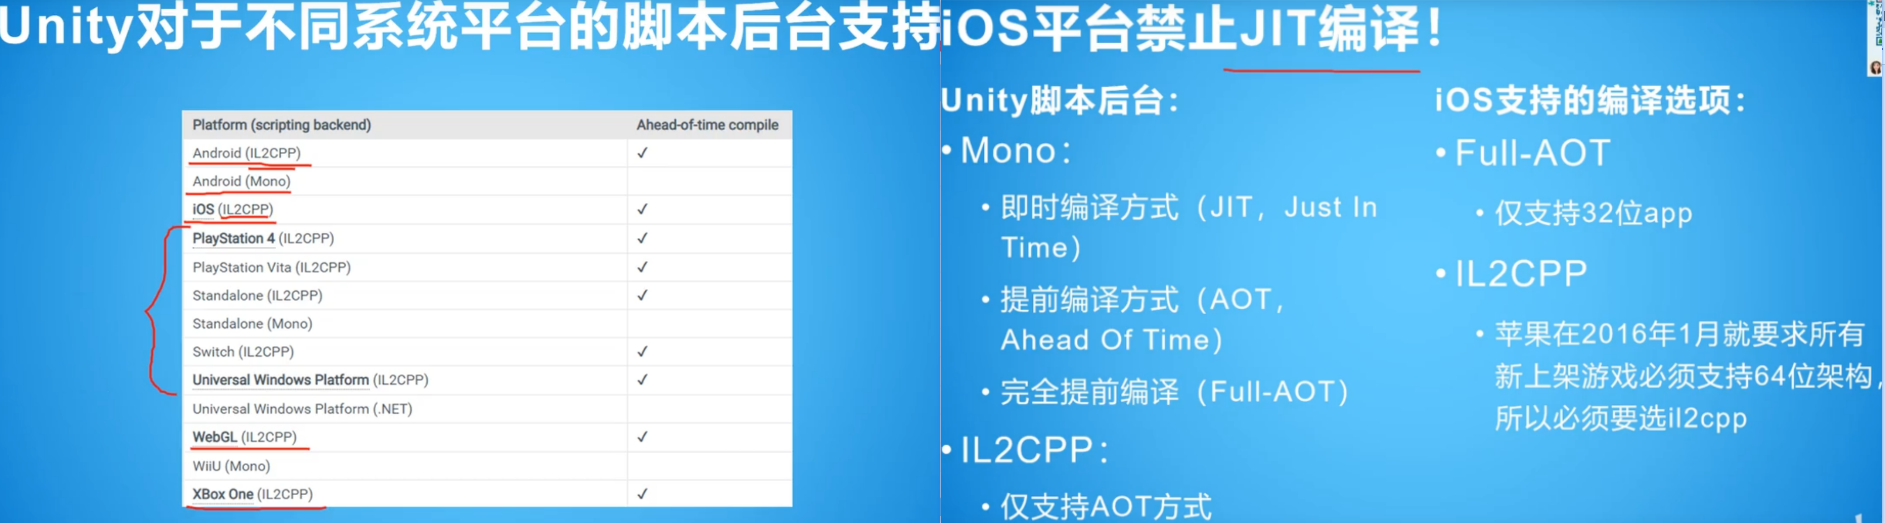
\includegraphics[width=.9\linewidth]{./pic/notes_20221125_094520.png}
\begin{itemize}
\item 最早IOS是支持MONO,但MONO只能支持32位,而且2016年后苹果要求必须64位。
\item IOS出于安全考虑,不允许JIT,而且因为禁止脚本为动态分配内存赋予执行权限,所以使用反射会有限制,只能静态编译,只能FULL AOT或者il2cpp,热更相对于安卓就比较麻烦。
\end{itemize}

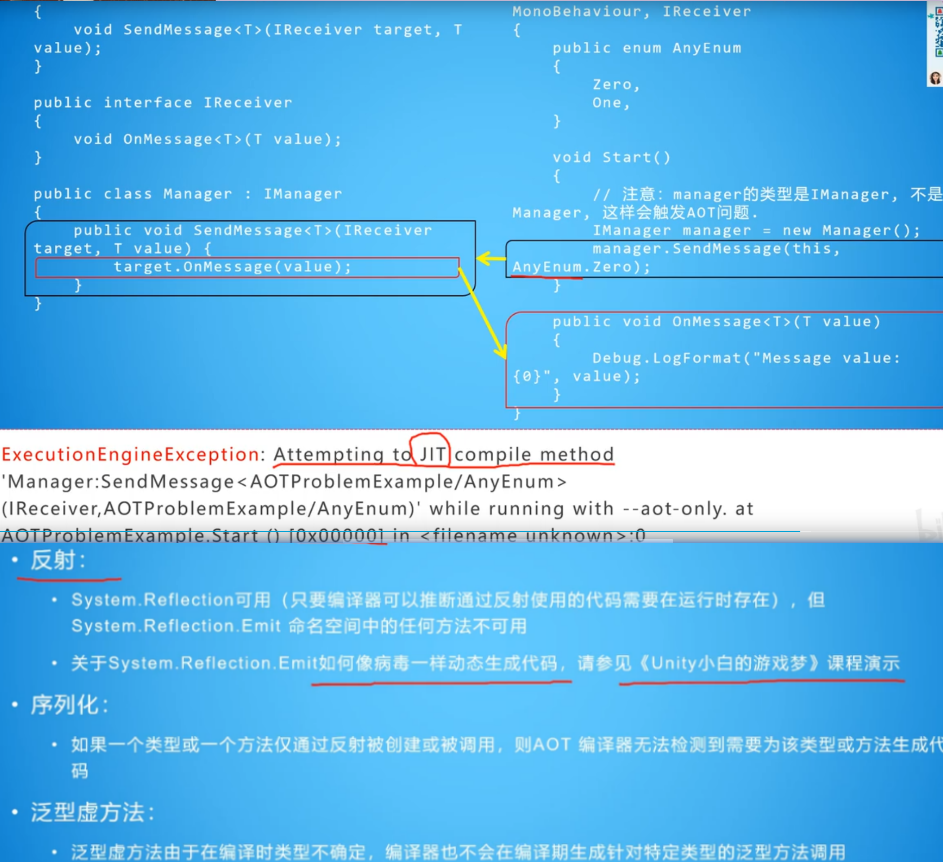
\includegraphics[width=.9\linewidth]{./pic/notes_20221125_094643.png}
\begin{itemize}
\item 在有泛型的情况下,代码很可能会报错,因为泛型T只有在执行的时候才知道自己的类型,属于动态的,所以静态编译会直接跳过这句代码,在运行的时候就会报错:尝试JIT的error.
\end{itemize}
% Emacs 27.2 (Org mode 8.2.7c)
\end{document}